\documentclass[bachelor,german]{hgbthesis}
% Zulässige Class Options: 
%   Typ der Arbeit: diplom, master (default), bachelor, praktikum 
%   Hauptsprache: german (default), english
%%------------------------------------------------------------

\graphicspath{{images/}}    % name of directory containing the images
\logofile{FHOOeIntl2014}			% name of PDF, remove or use \logofile{} for no logo
%\bibliography{literatur}  	% name of the BibTeX (.bib) file


%%%----------------------------------------------------------
\begin{document}
%%%----------------------------------------------------------

% Einträge für ALLE Arbeiten: --------------------------------
\title{3D Modellierung von Oberflächen mittels Marching Cubes
	Algorithmus und generische Darstellung mittels OpenGL}
\author{Peter P.\ Ortner}
\studiengang{Software Engineering}
\studienort{Hagenberg}
\abgabedatum{2015}{08}{01}	% {YYYY}{MM}{DD}

%%% zusätzlich für eine Bachelorarbeit: ---------------------
\nummer{S1210307080-A}   % XX...X = Stud-ID, z.B. 0310238045-A  
                        % (A = 1. Bachelorarbeit)
\semester{Sommersemester 2015} 
\gegenstand{Digitale Bildverarbeitung und Graphik} 
\betreuer{Werner ~Backfrieder, FH-Prof. DI Dr.} % oder \betreuerin{..}

%\strictlicense  % erzeugt restriktive Lizenzformel

%%%----------------------------------------------------------
\frontmatter
\maketitle
\tableofcontents
%%%----------------------------------------------------------

%\chapter{Vorwort} 	% engl. Preface






Dies ist \textbf{Version \hgbthesisDate} der \latex-Dokumentenvorlage für 
verschiedene Abschlussarbeiten an der FH Hagenberg, die mittlerweile auch 
an anderen Hochschulen im In- und Ausland gerne verwendet wird.

Das Dokument entstand ursprünglich auf Anfragen von Studierenden,
nachdem im Studienjahr 2000/01 erstmals ein offizieller
\latex-Grundkurs im Studiengang Medientechnik und -design an der
FH Hagenberg angeboten wurde. Eigentlich war die Idee, die bereits
bestehende \emph{Word}-Vorlage für Diplomarbeiten "`einfach"' in
\latex\ zu übersetzen und dazu eventuell einige spezielle
Ergänzungen einzubauen. Das erwies sich rasch als wenig
zielführend, da \latex, \va was den Umgang mit Literatur und
Graphiken anbelangt, doch eine wesentlich andere Arbeitsweise
verlangt. Das Ergebnis ist -- von Grund auf neu geschrieben und
wesentlich umfangreicher als das vorherige Dokument --
letztendlich eine Anleitung für das Schreiben mit \latex, ergänzt
mit einigen speziellen (mittlerweile entfernten) Hinweisen für \emph{Word}-Benutzer.
Technische Details zur aktuellen Version finden sich in Anhang \ref{ch:TechnischeInfos}.

Während dieses Dokument anfangs ausschließlich für die Erstellung
von Diplomarbeiten gedacht war, sind nunmehr auch  
\emph{Masterarbeiten}, \emph{Bachelor\-arbeiten} und \emph{Praktikumsberichte} 
abgedeckt, wobei die Unterschiede bewusst gering gehalten wurden.

Bei der Zusammenstellung dieser Vorlage wurde versucht, mit der
Basisfunktionalität von \latex das Auslangen zu finden und -- soweit möglich --
auf zusätzliche Pakete zu verzichten. Das ist nur zum Teil gelungen;
tat\-säch\-lich ist eine Reihe von ergänzenden "`Paketen"' notwendig, wobei jedoch
nur auf gängige Erweiterungen zurückgegriffen wurde.
Selbstverständlich gibt es darüber hinaus eine Vielzahl weiterer Pakete,
die für weitere Verbesserungen und Finessen nützlich sein können. Damit kann
sich aber jeder selbst beschäftigen, sobald das notwendige Selbstvertrauen und
genügend Zeit zum Experimentieren vorhanden sind.
Eine Vielzahl von Details und Tricks sind zwar in diesem Dokument nicht explizit
angeführt, können aber im zugehörigen Quelltext jederzeit ausgeforscht
werden.

Zahlreiche KollegInnen haben durch sorgfältiges Korrekturlesen und
konstruktive Verbesserungsvorschläge wertvolle Unterstützung
geliefert. Speziell bedanken möchte ich mich bei Heinz Dobler für
die konsequente Verbesserung meines "`Computer Slangs"', bei
Elisabeth Mitterbauer für das bewährte orthographische Auge und
bei Wolfgang Hochleitner für die Tests unter Mac~OS.

Die Verwendung dieser Vorlage ist jedermann freigestellt und an
keinerlei Erwähnung gebunden. Allerdings -- wer sie als Grundlage
seiner eigenen Arbeit verwenden möchte, sollte nicht einfach
("`ung'schaut"') darauf los werken, sondern zumindest die
wichtigsten Teile des Dokuments \emph{lesen} und nach Möglichkeit
auch beherzigen. Die Erfahrung zeigt, dass dies die Qualität der
Ergebnisse deutlich zu steigern vermag.

Der Quelltext zu diesem Dokument sowie das zugehörige
\latex-Paket sind in der jeweils aktuellen Version online
verfügbar unter
%
\begin{quote}
\url{www.fh-hagenberg.at/staff/burger/diplomarbeit/}
\end{quote}
%
oder auch unter
%
\begin{quote}
\url{http://elearning.fh-hagenberg.at/} \newline
im Kurs "`Anleitung/Vorlage für Master-/Bachelor-/Diplomarbeiten"'.
\end{quote}
%
Trotz großer Mühe enthält dieses Dokument zweifellos Fehler und Unzulänglichkeiten
-- Kommentare, Verbesserungsvorschläge und passende Ergänzungen
sind daher stets willkommen, am einfachsten per E-Mail direkt an mich:
\begin{center}%
\begin{tabular}{l}
\nolinkurl{wilhelm.burger@fh-hagenberg.at} \\
Dr.\ Wilhelm Burger \\
FH Hagenberg -- Digitale Medien\\
Austria
\end{tabular}
\end{center}

\noindent
Übrigens, hier im Vorwort (das bei Diplomarbeiten üblich, bei Bachelorarbeiten 
aber entbehrlich ist) kann man kurz auf die Entstehung  des Dokuments eingehen.
Hier ist auch der Platz für allfällige Danksagungen (\zB an den Betreuer, 
den Begutachter, die Familie, den Hund, ...), Widmungen und philosophische 
Anmerkungen. Das sollte man allerdings auch nicht übertreiben und sich auf 
einen Umfang von maximal zwei Seiten beschränken.




		% ggfs. weglassen

\chapter{Kurzfassung}

In der computergestützten Bildverarbeitung gibt es diverse Möglichkeiten für die Darstellung von dreidimensionalen Objekten. Die wohl am weitesten verbreitete Darstellungsform ist die polygonale Darstellung. Diese Form der Aufbereitung zerlegt ein gegebenes Objekte in Dreiecke. 
\\\\
Ein weiteres Verfahren ist die Methode der Modellierung via einer so genanten Voxel-Datenmenge. Jedoch birgt diese, im Bezug auf die digitale Verarbeitung, einige Nachteile gegenüber der polygonalen Darstellungsform. Vordergründige Probleme hierbei sind der vergleichsweise hohe Speicherverbrauch der Modelle, die Visualisierung benötigt länger und Objektmanipulationen erweisen sich als schwieriger.
\\\\
Da in der Medizin im Bereich der bildgebenden Systeme wie der Computertomografie von Natur aus solche Voxel-Modelle erzeugt werden, besteht die Anforderung auch diese nach Möglichkeit schnell und Aussagekräftig darzustellen.
\\\\
Um diesen Anforderungen an die Darstellung gerecht zu werden bietet sich der so genante Marching-Cubes Algorithmus an. Dieser ermöglicht es eine Voxel-Datenmenge in eine polygonale Darstellung zu überführen. 
		
\chapter{Abstract}

Considering the computer based image processing there are multiple possibilities to represent three-dimensional objects. The most common way to illustrate these objects is the polygonal approach. This approach fragments an object into triangles.
\\\\
An other possible procedure to model objects is to represent them as a voxel grid. But if we consider the ability to process this kind of representation we have to face some disadvantages. The main problems are: the model needs a comparatively high amount of disk space, it takes much longer to show the image and it is difficult to perform manipulations on the object.
\\\\
In the field of Medical imaging such as computed tomography creates such voxel models, these should be presented quickly and meaningfully.
\\\\
To implement these requirements on the presentation we have to transform voxel grids into polygon objects. The so called marching cubes algorithm can achieve this goal.
\\\\
This thesis gives a quick overview of the Marching Cubes Algorithm and tries to explain it in an easy way. To show the functionality it provides an C/C++ implementation of the Algorithm. It also provides the possibility to represent a generated model via OpgenGL and shows how to export a polygonal object as .stl File.			

%%%----------------------------------------------------------
\mainmatter         % Hauptteil (ab hier arab. Seitenzahlen)
%%%----------------------------------------------------------

\chapter{Einleitung}

\section{Aufgabenstellung}
In der medizinischen Diagnostik wird im Gegensatz zu CAD-Konstruktionen die dreidimensionale
Gestalt anatomischer Details aus Volumsbildern abgeleitet. Durch vorangegangene Segmentierung werden binäre Objekte erzeugt, d.h. das Objekt ist wie eine Lego-Figur aufgebaut. Mit dem Marching Cubes Algorithmus wird aus diesem binären Volumen eine Oberfläche, welche aus Dreiecken besteht, aufgebaut. Diese Oberfläche wird in einem binären STL-Format persistiert und anschließend mithilfe von generischem Rendering als 3D-Objekt dargestellt.\\\\
Anforderungen: C/C++ Implementierung des MC-Algorithmus (Matlab-Version vorhanden), Konversion in STL-Format, OpenGl Visualisierung.

\section{Motivation}
Da moderne Grafikchips auf die Darstellung von polygonalen Modellen ausgelegt sind, ist es sinnvoll, die aus der medizinischen Diagnostik erhaltenen Voxel-Modelle für spätere Verarbeitung in diese Form zu überführen. Ein weiterer Vorteil neben der vereinfachten Verarbeitung und Darstellung von Polygonen liegt in dem vergleichsweise geringen Speicherbedarf eines solchen Objektes.

\section{Zielsetzung}
Ziel dieser Arbeit ist es, die aus bildgebenden Verfahren der Medizin erhaltenden Voxel-Mengen mithilfe des Marching Cubes Algorithmus in eine polygonale Darstellung zu überführen. Als Input werden die Daten, welche von dem Programm Analyze 7.5\footnote{https://rportal.mayo.edu/bir/} erzeugt werden verwendet. Im Speziellen handelt es sich hierbei um die Formate Image (.img) und Header (.hdr). Die Voxel-Menge, welche in der Image-Datei abgelegt ist, wird ausgelesen und mithilfe des Marching Cubes Algorithmus in Polygone zerlegt. Nach erfolgreicher Umwandlung wird die erhaltene Datenmenge via OpenGL dargestellt. Des Weiteren soll das Modell als STL-Datei exportiert werden können. Die gesamte Umsetzung erfolgt in der Programmiersprache C++. 

\chapter{Allgemeine Einführung}

\section{Bildgebende Verfahren}
\begin{quote}
	''Die Medizinische Bildverarbeitung hat das Ziel, medizinische Bilder und Bildfolgen zur Unterstützung der medizinischen Diagnostik und Therapie aufzubereiten, zu analysieren und zu visualisieren.'' - \citep{MedBildVerarbeitung}
\end{quote}
Die verschiedenen medizinischen Verfahren können in die Art der erzeugten Bilddaten eingeteilt werden:
\begin{itemize}
	\item \textbf{Schnittbilder} z.B. mittels Computertomografie, Magnetresonanztomografie oder Röntgentomografie.
	\item \textbf{Projektionsbilder} z.B. durch ''klassisches'' Röntgen.
	\item \textbf{Oberflächenabbildungen} z.B. durch Rastertunnelmikroskop.
\end{itemize}
Da das Hauptaugenmerk dieser Arbeit liegt auf der aus den tomographischen Verfahren erhaltenden Schnittbildern, welche als sogenannte Voxel-Daten gespeichert werden. Ein vollständiges dreidimensionales Bild besteht aus mehreren solcher übereinandergelegten Schnittbildern.

\section{Volumengrafik}
Unter Volumengrafik versteht man in der Computergrafik die Darstellung von Objekten durch eine Menge von Voxeln. 
\\\\
Ein solches Voxel ist als ein einzelner Punkt in einem dreidimensionalen Objekt zu verstehen, welcher einen gewissen Isowert aufweist. Dieser Wert ist essentiell um z.B. bei den tomographischen Verfahren in der Medizin die festeren von den weicheren teilen eines Körpers zu unterscheiden (z.B. Knochen und Gewebe). In Abbildung \ref{fig:Voxelgitter} ist eine solche Voxel-Menge zusehen die verschiedenen Grauwerte der einzelnen Bildpunkte stellen dabei die unterschiedlichen Isowert dar.

\begin{figure}
	\centering
	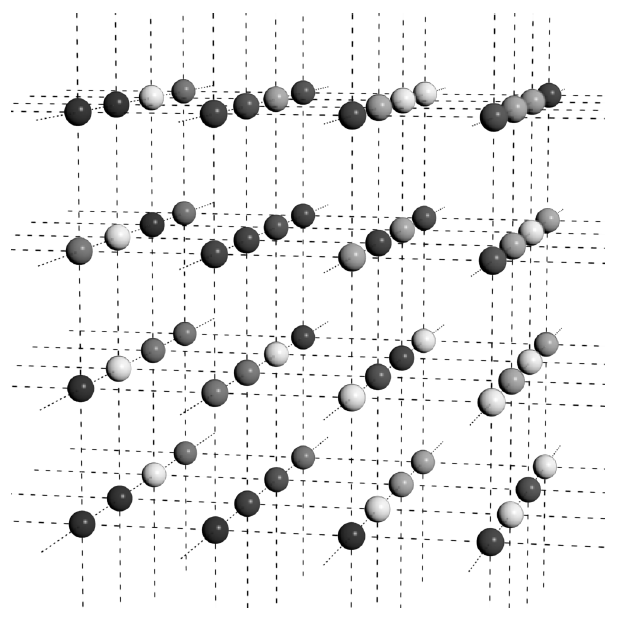
\includegraphics[width=.85\textwidth]{Voxelgitter}
	\caption{Ein Voxelgitter \citep{SeibtBak}.}
	\label{fig:Voxelgitter}
\end{figure}

\section{Marching Cubes}
Da der Marching Cubes Algorithmus das zentrale Element dieser Arbeit bildet wird hier seine Grundform wie sie in \citep{MCAlgo} beschrieben ist nochmals genau erörtert. 
\subsection{Formale Definition}
\begin{quote}
	''Der Marching Cubes Algorithmus ist ein Algorithmus um eine Isofläche $S_{c}$ eines Objektes, dass in einem Skalarfeld  $\varphi : \mathbb{R}^{n} \rightarrow \mathbb{R }$ beschrieben wird durch Dreiecke zu approximieren. Der Isowert c $\epsilon$ $ \mathbb{ R} $ beschreibt die gemeinsame Eigenschaft des Objektes wie z.B. gleiche Dichte, Temperatur oder emittierter Strahlung.''
\end{quote} \citep{WollmannBak}\\

\noindent Durch den Marching Cubes Algorithmus wird für eine Isofläche $S_{c}$ (s. \ref{mat:isoDef})
eine endliche Menge an Datenpunkten P $\subset \mathbb{R}^{n} \text{ x } \mathbb{R}$ zur Approximation von $S_{c}$ erzeugt (vgl. \citep{VisualHandbook}).

\begin{equation}
\label{mat:isoDef}
S_{c} := \{ \vartheta \text{ } \epsilon \text{ } \mathbb{R}^{n} \text{ | } \varphi(\vartheta) = c\}
\end{equation} 
\subsection{Funktionsweise}

Wie der Name des Algorithmus bereits sagt wird durch die Voxel-Menge ''marschiert''. Die Input-Menge des Algorithmus umfasst 8 aneinander grenzende Punkte der Voxel-Menge welche zusammen einen Würfel bilden sowie eines Schwellwerts für dem Isowert. Nach erfolgreicher Verarbeitung wird zum nächste Würfel gewandert (''marschiert'') bis die gesamte Datenmenge abgearbeitet wurde. 
\subsubsection{Vorbereitung}
Wie bereits erwähnt wird der Algorithmus für jeden einzelnen Würfel der gesamten Menge angewendet. Für ein besseres Verständnis zeigt Abbildung \ref{fig:Wuerfel} einen solchen Würfel (rot) in einem Voxelgitter.
\begin{figure}[H]
	\centering
	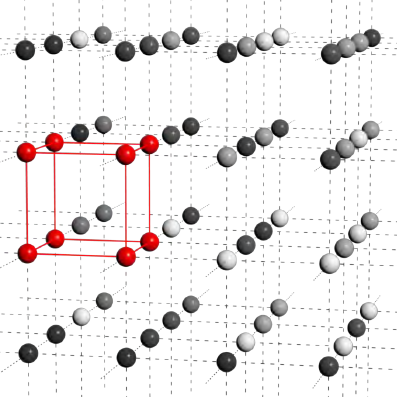
\includegraphics[width=.50\textwidth]{Wuerfel}
	\caption{Ein Wüfel im Voxelgitter \citep{SeibtBak}.}
	\label{fig:Wuerfel}
\end{figure}
\noindent Als erster Schritt im Algorithmus werden nun die Ecken und Kanten des Würfels für die spätere Verarbeitung indiziert (s. Abbildung \ref{fig:WuerfelIndizierung}).
\begin{figure}[H]
	\centering
	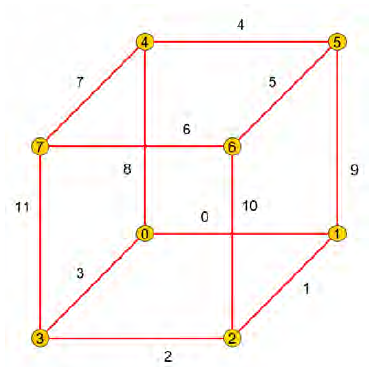
\includegraphics[width=.50\textwidth]{WuerfelIndizierung}
	\caption{Indizierung eines Würfels \citep{SeibtBak}.}
	\label{fig:WuerfelIndizierung}
\end{figure}

\noindent Jede Ecke des Würfels kann aufgrund seines Isowertes als Solide bzw. Transparent klassifiziert werden. Folglich sind aufgrund der Zwei möglichen Werte jeder Ecke $2^{8} = 256$ unterschiedliche Konfigurationen der Eingabemenge möglich. Jede dieser Konfigurationen kann als ein 8 Bit Muster dargestellt werden wobei gilt, dass jedes Bit \textit{i} bei welchem der Isowert \textit{$d_{i}$} des dazugehörigen Voxel einen gewissen Schwellwert \textit{c} überschreitet als binäre 0 interpretiert wird. Für die Werte kleiner gleich des Schwellwertes wird eine Binäre 1 angenommen.\\\\ Betrachtet man nun dieses Bitmuster als natürliche Zahl erhält man einen sogenannten Würfelindex zwischen 0  und 255 welcher für die weitere Verarbeitung essentiell ist.

\subsubsection{Verarbeitung}
Aufgrund der Symmetrie eines Würfels können durch Rotation bzw. Spiegelung die Anzahl der 255 möglichen Anordnungen der Voxeln auf 15 unterschiedliche Konfigurationen reduziert werden. Diese 15 Konfigurationen sind in Abbildung \ref{fig:MCPos} zu sehen.
\begin{figure}[H]
	\centering
	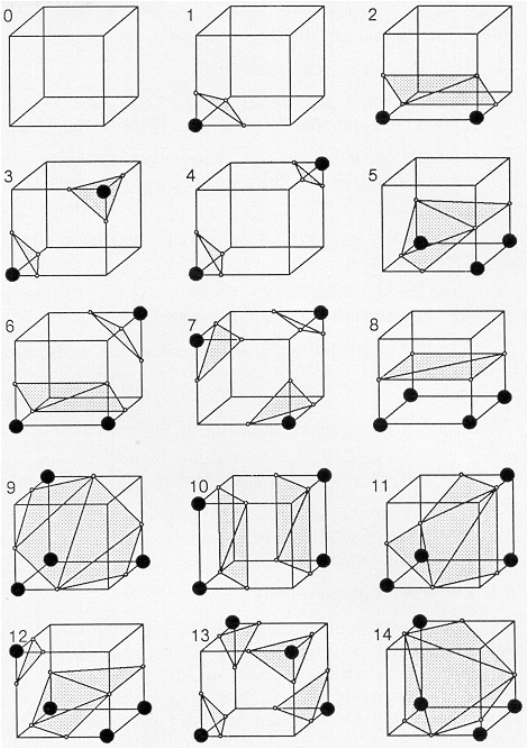
\includegraphics[width=.70\textwidth]{MCPos}
	\caption{Marching Cubes Grundkonigurationen \citep{MCAlgo}.}
	\label{fig:MCPos}
\end{figure}
\section{Dateiformate}
Die zu dieser Arbeit herangezogenen Dateiformate sind einerseits die von dem Softwarepaket Analyze\footnote{https://rportal.mayo.edu/bir/} verwendeten Image und Header Files sowie die sogenannte STereoLithography-Schnittstelle. 

\subsection{Image File (.img)}
Diese Datei ist vergleichsweise einfach aufgebaut und enthält ein Objekt bestehend aus (normalerweise) unkomprimierten Pixel Daten (vgl. \citep{AnalyzeFormat}). Jedes Pixel repräsentiert eine Voxel mit dem dazugehörigen Isowert. Das gesamte Objekt kann somit in eine 3x3 Matrix eingelesen und verarbeitet werde.

\subsection{Header File (.hdr)}
Diese Datei beschreibt die Ausmaße der Pixel-Datei sowie ihre Historie. (vgl. \citep{AnalyzeFormat}). \\\\
Die genaue Struktur nach \citep{AnalyzeFormat} ist in drei Teilbereiche aufgeteilt. Der erste Teil ist der sogenannte ''header key'' und beinhaltet allgemeine Informationen bezüglich der Datei (s. \ref{prog:headerKey}). Der zweite Teil beinhaltet Informationen bezüglich der Dimension der Image-Datei(s. \ref{prog:imageDim}. Der dritte und letzte Abschnitt hält Informationen bezüglich der Historie (s. \ref{prog:dataHist}).

\begin{program}[H]
	\caption{Header key als C-Struktur \citep{AnalyzeFormat}}
	\label{prog:headerKey}
	\begin{CCode}
struct header_key /* header key */
{ /* off + size */
	int sizeof_hdr /* 0 + 4 */
	char data_type[10]; /* 4 + 10 */
	char db_name[18]; /* 14 + 18 */
	int extents; /* 32 + 4 */
	short int session_error; /* 36 + 2 */
	char regular; /* 38 + 1 */
	char hkey_un0; /* 39 + 1 */
}; /* total=40 bytes */ 
	\end{CCode}
\end{program}

\begin{program}[H]
	\caption{Data history als C-Struktur \citep{AnalyzeFormat}}
	\label{prog:dataHist}
	\begin{CCode}
struct data_history
{ /* off + size */
	char descrip[80]; /* 0 + 80 */
	char aux_file[24]; /* 80 + 24 */
	char orient; /* 104 + 1 */
	char originator[10]; /* 105 + 10 */
	char generated[10]; /* 115 + 10 */
	char scannum[10]; /* 125 + 10 */
	char patient_id[10]; /* 135 + 10 */
	char exp_date[10]; /* 145 + 10 */
	char exp_time[10]; /* 155 + 10 */
	char hist_un0[3]; /* 165 + 3 */
	int views /* 168 + 4 */
	int vols_added; /* 172 + 4 */
	int start_field; /* 176 + 4 */
	int field_skip; /* 180 + 4 */
	int omax, omin; /* 184 + 8 */
	int smax, smin; /* 192 + 8 */
}; 
	\end{CCode}
\end{program}

\begin{program}[H]
	\caption{Image Dimension als C-Struktur \citep{AnalyzeFormat}}
	\label{prog:imageDim}
	\begin{CCode}
struct image_dimension
{ /* off + size */
	short int dim[8]; /* 0 + 16 */
	short int unused8; /* 16 + 2 */
	short int unused9; /* 18 + 2 */
	short int unused10; /* 20 + 2 */
	short int unused11; /* 22 + 2 */
	short int unused12; /* 24 + 2 */
	short int unused13; /* 26 + 2 */
	short int unused14; /* 28 + 2 */
	short int datatype; /* 30 + 2 */
	short int bitpix; /* 32 + 2 */
	short int dim_un0; /* 34 + 2 */
	float pixdim[8]; /* 36 + 32 */
	/*
	pixdim[] specifies the voxel dimensitons:
	pixdim[1] - voxel width
	pixdim[2] - voxel height
	pixdim[3] - interslice distance
	...etc
	*/
	float vox_offset; /* 68 + 4 */
	float funused1; /* 72 + 4 */
	float funused2; /* 76 + 4 */
	float funused3; /* 80 + 4 */
	float cal_max; /* 84 + 4 */
	float cal_min; /* 88 + 4 */
	float compressed; /* 92 + 4 */
	float verified; /* 96 + 4 */
	int glmax,glmin; /* 100 + 8 */
}; /* total=108 bytes */ 
	\end{CCode}
\end{program}

\subsection{STereoLithography (.stl)}
\begin{quote}
	''The STL (STereoLithography) file format, as developed by 3D Systems, has been widely used by most Rapid Prototyping (RP) systems and is supported by all major computer-aided design (CAD) systems.'' - \citep{STereoLithography}
\end{quote}
Eine STL-Datei besteht im Prinzip aus einer liste von Dreiecken. Jedes Dreieck wird durch seine drei Eckpunkte im Raum (jeweils x, y und z Position) sowie durch seinen Normalvektor beschrieben. Dies führt folglich zu einer Summe von 12 Werten pro Dreieck.\\
\\
Zum besseren Verständnis kann in Abbildung \ref{fig:ASCIISTL} der Aufbau einer solchen Datei als ASCII Darstellung betrachtet werden. 

\begin{figure}[H]
	\centering
	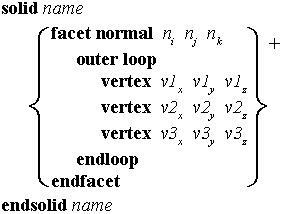
\includegraphics[width=.65\textwidth]{StL-ASCII}
	\caption{ASCII Darstellung des STL-Format \citep{STLFormat}.}
	\label{fig:ASCIISTL}
\end{figure}
\noindent Für ein besseres Verständnis hinsichtlich der Implementierung ist in Abbildung \ref{fig:BINARYSTL} der Binäre Aufbau des STL-Formates zu dargestellt. 
\begin{figure}[H]
	\centering
	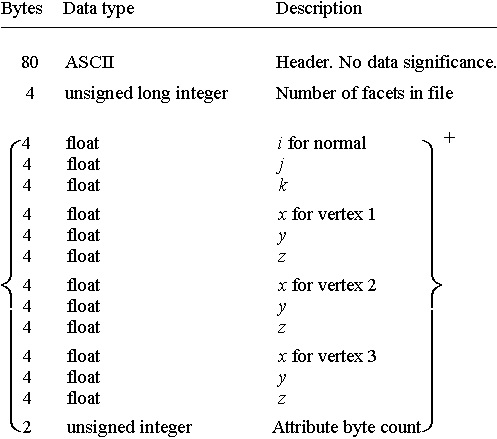
\includegraphics[width=.65\textwidth]{StL-binary}
	\caption{Binäre Darstellung des STL-Format \citep{STLFormat}.}
	\label{fig:BINARYSTL}
\end{figure}

\section{Computergrafik}
Computergrafik beschreibt das computergestützte Erstellen und Verarbeiten von Grafiken (vgl. \citep{ComputerGraphics}). In dieser Arbeit wird auf die Verarbeitung und insbesondere auf die Darstellung von dreidimensionalen Objekten als Polygon-Menge zurückgegriffen. Zu diesem Zweck bieten sich diverse Programmierschnittstellen wie OpenGL\footnote{https://www.opengl.org/}, Direct3D\footnote{https://msdn.microsoft.com/en-us/library/windows/desktop/bb153256(v=vs.85).aspx} oder AMD Mantle\footnote{http://www.amd.com/de-de/innovations/software-technologies/technologies-gaming/mantle} an, welche für Grafikausgaben genutzt werden können. Aufgrund der Aufgabenstellung wird in dieser Arbeit OpenGL verwendet.
\subsection{OpenGL}
\begin{quote}
	''OpenGL (for “Open Graphics Library”) is a software interface to graphics hardware.
	The interface consists of a set of several hundred procedures and functions
	that allow a programmer to specify the objects and operations involved in producing
	high-quality graphical images, specifically color images of three-dimensional
	objects.'' - \citep{OpenGLDoku}
\end{quote}
OpenGL ermöglicht eine verhältnismäßig einfache Plattform unabhängige Grafikprogrammierung. Da es sich um eine reine Grafikbibliothek handelt kümmert sich OpenGL nicht um die Verwaltung von Zeichenoberflächen, Renderkontexten oder weitere Puffer. Um OpenGL vernünftig mit einem Betriebssystem zu verwenden existieren daher verschiedene Bibliotheken. Die in dieser Arbeit verwendete Bibliothek ist QT. Die hierfür sind die Unabhängigkeit bezüglich Betriebssystem, die Aktualität der Bibliothek sowie die hohe Verbreitung dieser.
\chapter{Umsetzung}
Im Rahmen dieser Arbeit entstand ein in C++ geschriebenes Programm welches den Marching Cubes Algorithmus auf eine Voxelmenge anwendet und das Resultat via OpgenGL visualisiert. Des Weiteren ist es möglich das verarbeitete Model als STereoLithography (.stl) Datei zu exportieren.
\section{Marching Cubes}
\label{sec:mcUms}
Der Marching Cubes Algorithmus ist das Herzstück der entstandenen Applikation er ermöglicht die Umrechnung der gegebenen Voxel Datenmenge in eine polygonale Darstellung welche sich im später vergleichsweise einfach darstellen lässt.
\subsection{Allgemein}
Die Implementierung ist eine angepasst Version der von [ref] bereitgestellten Umsetzung. Die wesentlichen Änderungen sind die Auslagerung der Funktionen in eine eigenen Klasse und das verwenden anderer Datenstrukturen. Durch die Umstellung auf STL-Behälter und der daraus folgende Verzicht auf C-Strukturen welche zur Laufzeit immer neuen Speicher anfordern konnte die Geschwindigkeit enorm erhöht werde.
\subsection{Schnittstelle (Klasse)}
\begin{figure}[H]
	\centering
	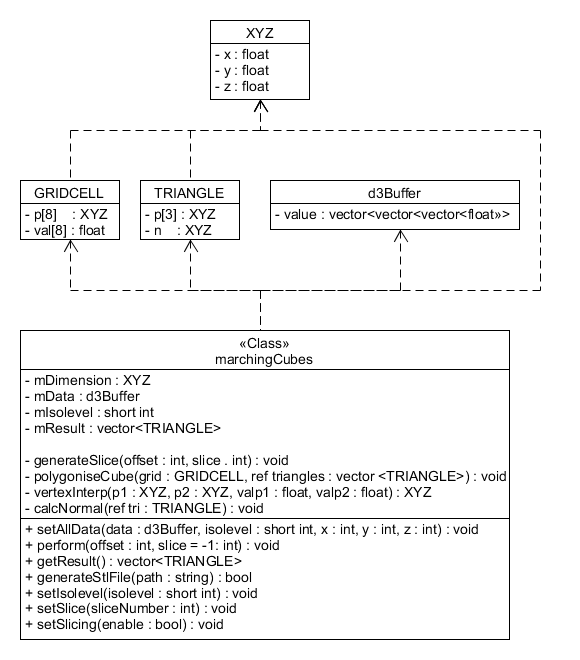
\includegraphics[width=.90\textwidth]{marchingCubes}
	\caption{UML-Diagramm der marchingCubes Klasse}
	\label{fig:marchingCubes}
\end{figure}

\subsubsection{Datentypen}
Neben den üblichen Datentypen wurden zur Vereinfachung komplexere Strukturen verwendet.\\
\begin{itemize}
	\item \textbf{XYZ} beschreibt einen Punkt im dreidimensionalen Raum.
	\item \textbf{GRIDCELL} ist die Repräsentation eines Voxel-Würfels. 
	\item \textbf{TRIANGLE} Repräsentiert ein Dreieck mithilfe seiner drei Eckpunkte und seiner Normalen.
	\item \textbf{3dBuffer} bildet ein Voxelgitter als dreidimensionalen Vektor im Speicher ab.
\end{itemize}

\subsubsection{Funktionen}
Um ein grundlegendes Verständnis zu bieten werden hier die öffentlichen Methoden der Klasse kurz beschrieben. 
\begin{itemize}
	\item \textbf{setAllData:} Da während der Laufzeit des Programmes nur eine Instanz der marchingCubes-Klasse instanziiert wird, ist es notwendig diese, wenn nötig, mit neuen Werten zu initialisieren. Es wird das gesamte Voxelgitter (data) sowie der zu verwendende Schwellwert (isolevel) für die Berechnung mitgegeben.
	\item \textbf{perform:} Diese Funktion führt den Marching Cubes Algorithmus auf dem zuvor via setAllData gesetzten Voxelgitter aus. Es bestehen zwei Möglichkeiten des Aufrufs. Zum Einen mit beiden Parameter und zum Anderen mit nur dem ersten (offset) Parameter. Bei der ersten Variante wird nur eine Scheibe des Voxelgitters betrachtet, wobei der erste Parameter die Dicke der Scheibe und der zweite die Position der Scheibe im Gitter kennzeichnet. Bei der zweiten Variante wird der gesamte Input betrachtet wobei Parameter ''offset'' die Schrittweite pro Würfel angibt. 
	\item \textbf{getResult:} Hier kann nach dem durchlaufen von perform das Ergebnis des Algorithmus abgegriffen werden. 
	\item \textbf{setIsolevel:} Hier kann der Schwellwert der Voxeln für den Algorithmus nachträglich verändert werden.
	\item \textbf{generateStl:} Das ausführen dieser Funktion persistiert das Ergebnis des Marching Cubes Algorithmus als .stl Datei.
\end{itemize}
\subsubsection{Verwendung}
Im Programm \ref{prog:MCVerw} ist die Verwendung der Klasse exemplarisch dargestellt.
\begin{program}[H]
	\caption{Verwendung der marchingCubes Klasse}
	\label{prog:MCVerw}
	\begin{CCode}
		int main(){
			marchingCubes *mc = new marchingCubes();
			// set the voxelgrid and the treshold
			mc->setAllData(getRawData(), getIsolevel()); 
			// performs the marching cubes algorithmus on the entire voxelgrid
			mc->perform(getOffset()); 		
			// performs the algorithmus on just a slice of the voxelgrid 
			mc->perform(getOffset(), getSlice()); 
			showPolygons(mc->getResult()); 
			delete(mc);
			return 0;	
		}
	\end{CCode}
\end{program}
\section{File Formate}
Wie bereits im Kapitel \ref{sec:DateiEinf} erwähnt wurden für die Umsetzung die Dateiformate von Analyze 7.5 (.img und .hdr) sowie das STereoLithography (.stl) Format verwendet.
\subsection{Allgemein}
Um eine unnötige Komplexität zu vermeiden wurden für die Analyze-Formate nur lesender und für das STereoLithography Format nur schreibende Zugriff implementiert. Hier bieten sich für spätere Erweiterungen viele Möglichkeiten bezüglich Import/Export (auch für weitere Formate). 
\subsection{Image File (.img)}
Um das Image File auszulesen müssen vorher die Dimensionen des Voxelgitters bekannt sein.  Diese Information erhält man aus dem Header File. Sind die Dimensionen bekannt können mithilfe einer dreifach geschachtelten for-Schleife die einzelnen Voxel-Werte in eine entsprechende Datenstruktur (z.B. dreidimensionales Array) ausgelesen werden. In \citep{AnalyzeFormat} ist eine beispielhafte Implementierung gegeben. Diese wurde für den Prototyp angepasst und integriert.
\subsection{Header File (.hdr)}
Diese Datei ist wie bereits in Kapitel \ref{sec:DateiHead} beschrieben aufgebaut. Auch hier ist in \citep{AnalyzeFormat} eine beispielhafte Implementierung gegeben welche für die Verwendung angepasst und erweitert wurde.
\subsection{STereoLithography (.stl)}
In Abbildung \ref{fig:BINARYSTL} ist bereits der binäre Aufbau einer STL-Datei abgebildet. Die Implementierung (Programm \ref{prog:generateSTL}) richtet sich daher genau an diesen formalen Aufbau.
\begin{program}[H]
	\caption{Generierung einer STL-Datei}
	\label{prog:generateSTL}
	\begin{CCode}
		bool fileHandler::CreateStl(std::string path){
			FILE *fptr = NULL;
	
			int sizeResult = mResult.size();
			fprintf(stderr, "Writing triangles ...\n");
			if ((fptr = fopen(path.c_str(), "a+b")) == NULL) {
				fprintf(stderr, "Failed to open output file\n");
				return false;
			}
			char fileHeader[81] = "solid Test Head";
			char bytes[3] = { 0x00, 0x00 };
			fwrite(&fileHeader, sizeof(fileHeader)-1, 1, fptr);
			fwrite(&sizeResult, sizeof(int), 1, fptr);
			for (int i = 0; i < mResult.size(); i++) {
				fwrite(&mResult[i].n, sizeof(float), 3, fptr);
				for (int k = 0; k < 3; k++)  {
					fwrite(&mResult[i].p[k], sizeof(float), 3, fptr);
				}
				fwrite(bytes, 2, 1, fptr);
			}
			fclose(fptr);
			return true;
		}
	\end{CCode}
\end{program}
\subsection{Schnittstelle (Klasse)}
\begin{figure}[H]
	\centering
	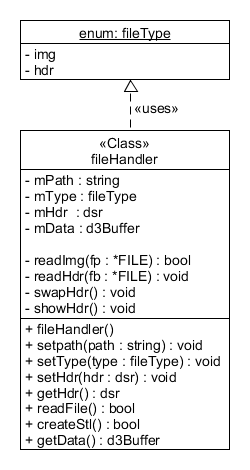
\includegraphics[width=.60\textwidth]{fileHandler}
	\caption{UML-Diagramm der fileHandler Klasse}
	\label{fig:fileHandler}
\end{figure}
\subsubsection{Datentypen}
\begin{itemize}
	\item \textbf{fileType} repräsentiert den zu verarbeitenden Dateityp als Enumeration (img bzw. hdr) 
	\item \textbf{dsr} ist die in Kapitel \ref{sec:DateiHead} beschriebene Repräsentation des Header-Formates als C-Struktur.
	\item \textbf{d3Buffer} wurde bereits im vorhergegangenen Abschnitt (\ref{sec:mcUms}) beschrieben.
\end{itemize}
\subsubsection{Funktionen}
Es folgt ein Überblick der öffentlichen Methoden dieser Klasse.
\begin{itemize}
	\item \textbf{fileHandler} der Konstruktor der Klasse initialisiert die Datenkomponenten für die spätere Verwendung.
	\item \textbf{setPath} setzt den Pfad zur verwendeten Datei.
	\item \textbf{setType} spezifiziert welche Dateityp von der Instanz dieser Klasse verwaltet werden soll.
	\item \textbf{setHdr:} Handelt es sich um eine Image-Datei sind dieser die Informationen aus der dazugehörigen Header-Datei mitzuteilen. 
	\item \textbf{getHdr:} Hier können nach dem Auslesen eines Header-File die erhaltenen Informationen abgegriffen werden. 
	\item \textbf{readFile:} Nach dem setzen von des Pfades und des Dateityps kann hier die entsprechende Datei ausgelesen werden.
	\item \textbf{createStl:} Ermöglicht das Erstellen einer .stl Datei aus den vom Marching Cubes Algorithmus gewonnen Dreiecken. 
	\item \textbf{getData:} Nach dem Auslesen einer Image-Datei können hier die erhaltenen Daten abgegriffen werden.
\end{itemize}
\subsubsection{Verwendung}
In Programm \ref{prog:fileClass} ist die beispielhafte Verwendung der fileHandler-Klasse skizziert.
\begin{program}[H]
	\caption{Verwendung der fileHandler-Klasse}
	\label{prog:fileClass}
	\begin{CCode}
		int main(){
			fileHandler *hdrFile = new fileHandler();
			fileHandler *imgFile = new fileHandler();
			
			// set the filetype
			hdrFile->setType(hdr);
			imgFile->setType(img);
			
			// set the file path
			hdrFile->setPath(ui->headerPath->text().toStdString());
			imgFile->setPath(ui->imagePath->text().toStdString());
			
			// read the header file
			hdrFile->readFile();
			// set the header for the image file
			imgFile->setHdr(hdrFile->getHdr());
			// read the image file
			imgFile->readFile();
			
			// get the image data and pass it to the marching cubes algorithm
			marchingCubes->setData(imgFile->getData());
			
			delete(hdrFile);
			delete(imgFile);
			return 0;	
		}
	\end{CCode}
\end{program}
\section{OpenGL}
Für die grafische Aufbereitung des generierten polygonalen Objektes wird wie bereits mehrfach erwähnt OpenGL verwendet. Um eine möglichst große Unabhängigkeit bezüglich des gewählten Betriebssystemes zu gewährleisten wurde QT als Schnittstelle zwischen System und OpenGL gewählt.
\subsection{Allgmein}
Die Implementierung ermöglicht die Darstellung des generierten Objektes, das bewegen um die Achsen via Maus sowie das Zoomen via Mausrat.
\subsection{Schnittstelle (Klasse)}
\begin{figure}[H]
	\centering
	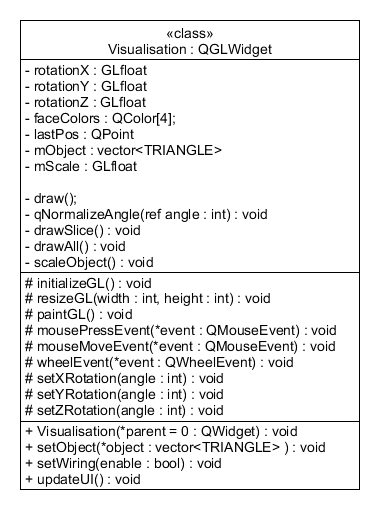
\includegraphics[width=.70\textwidth]{visualisation}
	\caption{UML-Diagramm der Visualisation Klasse}
	\label{fig:visualisation}
\end{figure}
\subsubsection{Funktionen}
\begin{itemize}
	\item \textbf{Visualisation:} Erstellen der Zeichenoberfläche.
	\item \textbf{setObject:} Setzen des zu zeichnenden Objektes.
	\item \textbf{setWiring:} Ermöglicht das hin -und herschalten zwischen den beiden Polygonmodi GL\_LINE und GL\_FILL (s. Abbildung \ref{fig:UIWiring}).
	\item \textbf{updateUI:} Manuelles update der Zeichenfläche z.B. nach setWiring oder setObjekt um die Änderungen für den Benutzer sichtbar zu machen.
\end{itemize}
\subsubsection{Verwendung}
Die Verwendung dieser Klasse ist vergleichsweise einfach. Eine beispielhafte Implementierung ist in Programm \ref{prog:VisVerw} zu finden.
\begin{program}
	\caption{Exemplarische Verwendung der Visualisation Klasse}
	\label{prog:VisVerw}
	\begin{CCode}
		int main(){
			Visualisation vi = new Visualisation();
			// set the polygon object (result of the marching cubes algorithm)
			vi->setObject(marchingCubes->getResult());
			// update ui for the user
			vi->updateUI;
			// enable wiring (set polygon mode to GL\_LINE)
			vi->setWiring(true);
			// update ui for the user
			vi->updateUI;
			delete(vi);
		} 
	\end{CCode}
\end{program}

\section{Benutzeroberfläche}
In diesem Abschnitt wird auf die Funktionen der Benutzeroberfläche (UI) des entstandenen Prototypen eingegangen. Erstellt wurde diese mithilfe des QT-Designers. Um eine einfache Benutzung zu gewährleisten wurde sie möglichst schlicht gehalten.

\subsection{Allgemeiner Aufbau}

\begin{figure}[H]
	\centering
	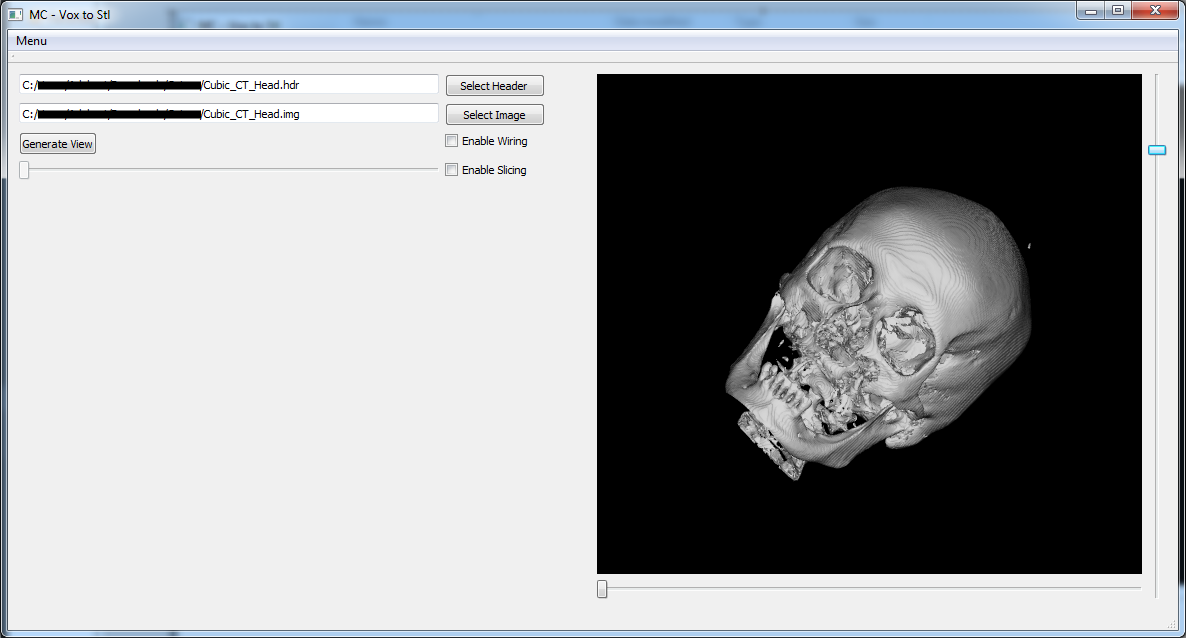
\includegraphics[width=1.0\textwidth]{UI1}
	\caption{Übersicht der Benutzeroberfläche}
	\label{fig:UI1}
\end{figure}
\subsection{Slicing}
Die Schaltfläche ''Enable Slicing'' ermöglicht die Darstellung einer einzelnen Scheibe des gesamt Objektes. Durch das Aktivieren der Checkbox wird auch der Regler links Aktiviert. Mithilfe von diesem kann das zu betrachtende Scheibenelement verschoben werden. Des Weiteren ändert sich die Funktionalität des unteren Reglers von der Regulierung der Polygongröße zur Regulierung der Dicke der Scheibe.\\
\\
Vorteil dieser Darstellungsform ist das mit aktivem Slicing das Innenleben eines Objektes betrachtet werden kann.\\
\\
Das Benutzerinterface mit Aktiviertem Slicing ist in Abbildung \ref{fig:UISlicing} zu sehen.
\begin{figure}[H]
	\centering
	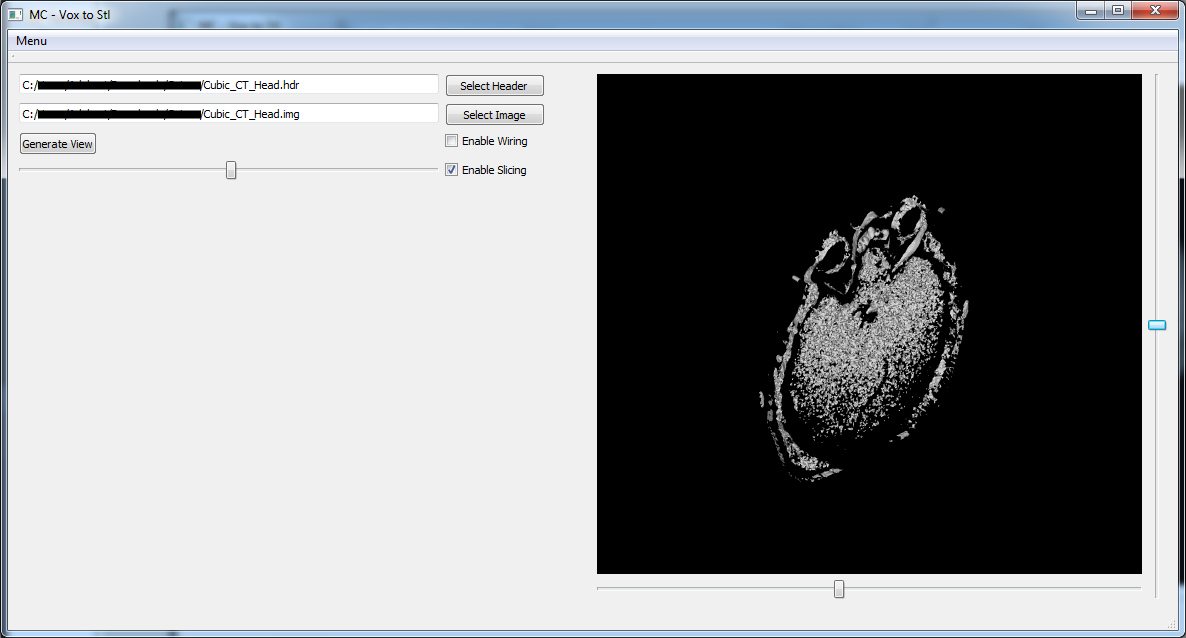
\includegraphics[width=1.0\textwidth]{UISlicing}
	\caption{Programm Slicing aktiviert}
	\label{fig:UISlicing}
\end{figure}
\subsection{Wiring}
Durch Aktivieren der Checkbox ''Enable Wiring'' kann das Drahtgittermodell des Objektes betrachtet werden. Diese Darstellung ermöglicht es die polygonale Struktur des Objektes besser zu erkennen. In Abbildung \ref{fig:UIWiring} ist ein Objekt mit aktiven Wiring zu sehen.
\begin{figure}[H]
	\centering
	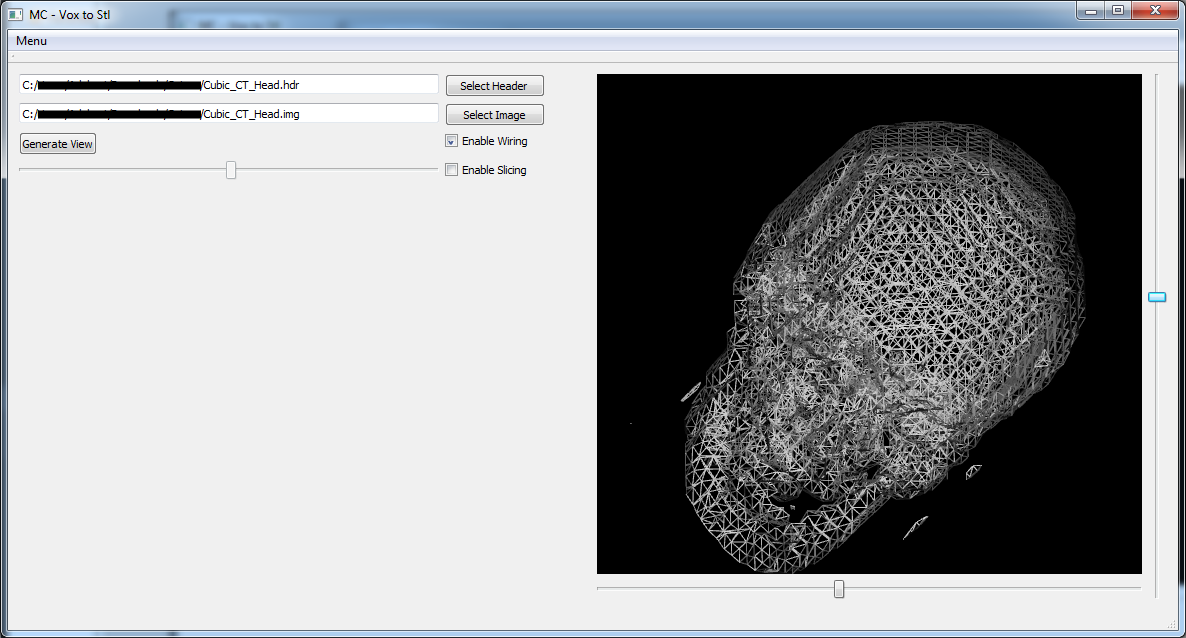
\includegraphics[width=1.0\textwidth]{UIWiring}
	\caption{Programm Wiring aktiviert}
	\label{fig:UIWiring}
\end{figure}
\chapter{Zusammenfassung und Ausblick}
Das Ziel dieser Arbeit war die Implementierung des von \citep{MCAlgo} vorgestellten Marching Cubes Algorithmus sowie die Darstellung des generierten polygonalen Modelles via OpenGL. Des Weiteren sollte es möglich sein die generierten Objekte als STereoLithography Datei zu exportieren da dies ein weit verbreitetes Format darstellt und von vielen Programmen unterstützt wird.\\
\\
In diesem Teil der Arbeit werden nun die Ergebnisse der Entwicklung dieser Applikation diskutiert. Außerdem wird kurz auf mögliche Erweiterungen und Verbesserungen welche nicht in die Umsetzung eingeflossen sind eingegangen.

\section{Ergebnisse}

\section{Erweiterungen}
\chapter{Literaturverzeichnis}
\bibliography{literatur}

%%%----------------------------------------------------------
%%%Anhang
%\appendix
%\chapter{Inhalt der CD-ROM}
\label{app:cdrom}

\paragraph{Format:} 
CD-ROM, Single Layer, ISO9660-Format%

\section{PDF-Dateien}
\begin{FileList}{BA1/}
	%\fitem{_DaBa.dvi} Gesamtdokument (DVI-File, ohne Grafiken)
	\fitem{_DaBa.pdf} Bachelorarbeit mit Instruktionen (Gesamtdokument)%
\end{FileList}


\section{\latex-Dateien}

\begin{FileList}{BA1/MarchingCubesLaTeX/}
	\fitem{_DaBa.tex} Diplom-/Bachelorarbeit (Hauptdokument) %
	\fitem{kurzfassung.tex} Kurzfassung %
	\fitem{abstract.tex} Abstract %
	\fitem{einleitung.tex} Kapitel 1 %
	\fitem{einfuehrung.tex} Kapitel 2 %
	\fitem{umsetzung.tex} Kapitel 3 %
	\fitem{zusammenfassung.tex} Kapitel 4 %
	\fitem{anhang_a.tex} Anhang A ((Inhalt CD-ROM) %
	\fitem{literatur.bib} Literatur-Datenbank (BibTeX-File)
\end{FileList}

\section{Style/Class-Dateien}

\begin{FileList}{BA1/MarchingCubesLaTeX/}
	\fitem{hgbthesis.cls} LaTeX Class-Datei für Master- und Bachelorarbeiten
	\fitem{hgb.sty} LaTeX Style-Datei für alle Hagenberg-Dokumente
\end{FileList}


\section{Implementierung}

\begin{FileList}{BA1/MarchingCubesVisualisation}
	\fitem{/Release} Beispielprogramm und benötigte .dll Dateien
	\fitem{marchingCubes.h} Klassendefinition für die Marching Cubes Klasse
	\fitem{marchingCubes.cpp} Implementierung des Marching Cubes Algorithmus
	\fitem{fileHandler.h} Klassendefinition für die Dateibearbeitung
	\fitem{fileHandler.cpp} Implementierung für die Dateibearbeitung
	\fitem{visualisation.h} Klassendefinition für die OpgenGL Komponente
	\fitem{visualisation.cpp} OpenGL Komponente
	\fitem{mainwindow.h}  Header File für die Verwaltung der Benutzeroberfläche
	\fitem{mainwindow.cpp} Kopplung von Benutzeroberfläche und Implementierung 
	\fitem{mainwindow.ui} Benutzeroberfläche (QT-Designer)
	\fitem{main.cpp} main Funktion der Applikation
	\fitem{dbh.h} C-Struktur für das .hdr Format
	\fitem{tabels.h} Lookuptabels für den Marching Cubes Algorithmus
	\fitem{MCV.pro} QT5 Projekt
	
\end{FileList}

\section{Sonstiges}

\begin{FileList}{BA1/MarchingCubesLaTeX/images}
	\fitem{*.jpg, *.png} Original Rasterbilder %
\end{FileList}

\begin{FileList}{BA1/MarchingCubesLaTeX/umlDiagrams}
	\fitem{*.uxf} Original UML-Diagramme
\end{FileList}	% Technische Ergänzungen
%\chapter{Inhalt der CD-ROM/DVD}
\label{app:cdrom}

\paragraph{Format:} 
		CD-ROM, Single Layer, ISO9660-Format%
\footnote{Verwenden Sie möglichst ein Standardformat, bei DVDs natürlich
eine entsprechende andere Spezifikation.}


\section{PDF-Dateien}
\begin{FileList}{/}
%\fitem{_DaBa.dvi} Gesamtdokument (DVI-File, ohne Grafiken)
\fitem{_DaBa.pdf} Diplom- oder Bachelorarbeit mit Instruktionen (Gesamtdokument)
\fitem{_PrBericht.pdf} Praktikumsbericht (verkürzte Version der Bachelorarbeit) %
\end{FileList}


\section{\latex-Dateien}

\textbf{Achtung:} Die folgende Auflistung soll nur den Gebrauch dieser Vorlage erleichtern. Es ist bei einer Diplom- oder Bachelorarbeit \ia\ \emph{nicht} notwendig, die zugehörigen \latex-Dateien aufzulisten (wohl aber projektbezogene Dateien, Ergebnisse, Bilder, Kopien von Online-Literatur etc.)!

\begin{FileList}{/}
\fitem{_DaBa.tex} Diplom-/Bachelorarbeit (Hauptdokument) %
\fitem{_PrBericht.tex} Praktikumsbericht (verkürzte Version der Bachelorarbeit) %
\fitem{vorwort.tex} Vorwort %
\fitem{kurzfassung.tex} Kurzfassung %
\fitem{abstract.tex} Abstract %
\fitem{einleitung.tex} Kapitel 1 %
\fitem{diplomschrift.tex} Kapitel 2 %
\fitem{latex.tex} Kapitel 3
\fitem{abbildungen.tex} Kapitel 4 %
\fitem{formeln.tex} Kapitel 5 %
\fitem{literatur.tex} Kapitel 6 %
\fitem{drucken.tex} Kapitel 7 %
\fitem{word.tex} Kapitel 8 %
\fitem{schluss.tex} Kapitel 9 %
\fitem{anhang_a.tex} Anhang A (Source Code) %
\fitem{anhang_b.tex} Anhang B (Inhalt CD-ROM) %
\fitem{anhang_c.tex} Anhang C (Liste der Änderungen) %
\fitem{anhang_d.tex} Anhang D (LaTeX-Quellcode) %
\fitem{messbox.tex} Messbox zur Druckkontrolle %
\fitem{literatur.bib} Literatur-Datenbank (BibTeX-File)
\end{FileList}

\section{Style/Class-Dateien}

\begin{FileList}{/}
\fitem{hgbthesis.cls} LaTeX Class-Datei für Master- und Bachelorarbeiten
\fitem{hgbtermreport.cls} LaTeX Class-Datei für Semesterberichte
\fitem{hgb.sty} LaTeX Style-Datei für alle Hagenberg-Dokumente
\end{FileList}


\section{Sonstiges}

\begin{FileList}{/images}
\fitem{*.ai} Original Adobe Illustrator-Dateien %
\fitem{*.fh11} Original Macromedia Freehand-Dateien %
\fitem{*.jpg, *.png} Original Rasterbilder %
%\fitem{*.eps} Bilder und Grafiken im EPS-Format%
%\fitem{fonts-bakoma/} BaKoMa TrueType Fonts %
\end{FileList}
	% Inhalt der CD-ROM/DVD
%\chapter{Chronologische Liste der Änderungen}


\begin{sloppypar}
\begin{description}
%
\item[2002/01/07]
\verb!\newfloat{program}! repariert (auch ohne Chapter). Dank an Werner Bailer!
%
\item[2002/03/06]
Copyright-Notice an internat.\ Standard angepasst. Dank an Karin Kosina!
%
\item[2002/07/28]
"`Studiengang"' $\rightarrow$ "`Diplomstudiengang"'
%
\item[2003/08/24]
Neues Macro: \verb!\Messbox{breite}{hoehe}! -- zur Kontrolle der 
Druckgröße ohne PS-Datei. Erweiterungen für Bakkalaureatsarbeiten
%
\item[2005/04/09]
Diverse Korrekturen: Captions von Tabellen nach oben gesetzt. 
\texttt{caption} auf neue Versionen adaptiert.
\texttt{subfigure} wird nicht mehr verwendet
%
\item[2006/01/20]
Adaptiert zur Verwendung als Praktikumsbericht 
(2.\ Bakk.-Arbeit)
%
\item[2006/03/24]
Fehler in \verb!\erklaerung! beseitigt (Dank an David Schwingenschlögl)
%
\item[2006/04/06]
Verwendung von T1-Fontencoding zur besseren Silbentrennung bei 
Umlauten etc.
%
\item[2006/06/21]
Neu: Bachelorstudiengang / Masterstudiengang.
Literaturverweise auf Bakk-Arbeiten.
\texttt{upquote.sty} eliminiert (Problem mit TS1-Kodierung).
Verwende Komma (statt Punkt) als Trennzeichen in Dezimalzahlen.
%
\item[2006/09/14]
Anmerkungen zum Thema Plagiarismus.
%
\item[2007/07/16]
Ergänzungen für Code-Listings (listings) und Algorithmen 
(\texttt{algorithmicx}).
BiBTeX-Datei aufgeräumt, Verwendung der Literaturformate 
verbessert.
Komma (statt Punkt) als Trennzeichen in Dezimalzahlen wieder 
entfernt.
Verwendung der \texttt{ae}-Fonts eliminiert (\texttt{cm-super} Fonts müssen 
installiert sein, ab MikTeX 2.5). 
Beispiel für Ersetzung in EPS-Dateien mit \texttt{psfrag}.
%
\item[2007/10/04]
Version 5.90: Das Laden der Pakete \verb!inputenc! (Option \texttt{latin}) und 
\verb!graphicx! (Option \texttt{dvips})
aus der Hauptdatei in die \texttt{sty}-Datei übertragen; \texttt{upquote} funktioniert nun.
Paket \texttt{eurosym} ergänzt für Euro-Symbol (Anregung von Andreas 
Doubrava).
Problem mit \texttt{color}-package repariert (gerasterter PDF-Ausdruck).
Hinweise bzgl.\ Literatur ergänzt (\texttt{month}, \texttt{edition}),
BibTeX-Datei gesäubert.
Hinweis zum Einfügen von vertikalem Abstand zwischen Absätzen.
Mathematik aufgeräumt, Verwendung von \texttt{amsmath}, 
Fallunterscheidungen.
Diverse Änderungen bei Tabellen und Programmkode.
Beispiele für BibTeX-Angaben von Spezialquellen: Audio-CDs, 
Videos, Filme. Einbinden von Dateien mit \verb!\include{..}!
Neue Datei: \verb!_SimpleReport.tex! für kurze Reports (Projekte etc.).
%
\item[2007/11/11]
Version 5.91: Hinweise zur Einstellung der Output-Profile in
TexNicCenter, Inverse Search Einstellung in YAP im Anhang.
%
\item[2008/04/01]
Version 6.00beta -- kompletter Umbau!
Auslagerung der Doku\-menten-relevanten Teile in eine eigene 
\emph{class}-Datei (\texttt{hgbthesis.cls}) mit Optionen.
Die neue Style-Datei \texttt{hgb.sty} ist nun unabhängig vom 
Dokumententyp und nicht mehr kompatibel mit älteren Versionen!
Die Liste der Änderungen ist jetzt in der Datei \verb!_ChangeLog.tex!
(DIESE Datei) und diese wird im Anhang eingebunden.
Heading-Style auf Sans Serif geändert (ohne grausliche "`Caps"').
%
\item[2008/05/22]
Neue Vorlage für Technical Reports (Klasse \texttt{hgbreport.cls}).
Spracheinstellung nunmehr mit \texttt{babel}-Paket, Hauptsprache
des Dokuments kann als Option der Klasse angegeben werden.
Sprachumschaltung innerhalb des Dokuments funktioniert nun
richtig. Mit der Sprachoption \texttt{german} wird automatisch die neue deutsche 
Orthographie (\texttt{ngerman}) verwendet.
\texttt{babelbib} wird zur Formatierung des Literaturverzeichnisses
verwendet (neue BibTeX-Style-Optionen!).
Header werden nunmehr mit \texttt{fancyhdr}-Paket erzeugt.
Versionsnummerierung von \texttt{.cls} und \texttt{.sty} Files wird beendet 
(ab jetzt gilt: \emph{Datum} = \emph{Version}). 
%
\item[2008/06/10]
Neues Listing-Environment \texttt{PhpCode}; bei allen Listing-Eviron\-ments ist nun 
\texttt{mathescape=false} (kein Math-Mode nach \verb!$!). 
Bug bei Sprachumschaltung auf \texttt{ngerman} beseitigt.
%
\item[2008/08/15]
Diverse Kleinigkeiten in Literaturangaben überarbeitet (Dank an Norbert Wenzel), Spracheinstellung vereinheitlicht, Umlaute in \texttt{.bib}-Datei ersetzt.
%
\item[2008/10/15] 
Zusätzliche Hinweise zur MikTeX-Installation (Windows) sowie LaTeX unter Mac OS~X und Linux.
Liste der Abkürzungen ergänzt.%
\item[2008/11/15] 
Diverse Schreibfehler korrigiert (Dank an Silvia Fuchshuber). Hinweis auf 
\texttt{sloppypar}-Umgebung.
%
\item[2008/12/09] 
BibTeX-Tools: neuer Hinweis auf JabRef ergänzt, BibEdit entfernt (ist nicht mehr auffindbar).
%
\item[2009/02/09]
\texttt{hgb.sty}: Option "`\texttt{spaces}"' zu \texttt{url}-Package ergänzt (ermöglicht gezielten Zeilenumbruch in URLs). 
Im allgemeinen Setup für \texttt{listings}: \texttt{keepspaces=true};
Obsoletes Environment \texttt{sourcecode} deaktiviert.
Escape-Mode für \texttt{LaTeXCode}-Umgebung geändert.
\verb!_DaBa.tex!: Hinweis auf die Verwendung von \verb!\urldef! für die Angabe von URLs in Captions. \texttt{diplom} (statt \texttt{master}) als Standard-Dokumententyp in \verb!_DaBa.tex! ("`Diplomarbeit"'). Neuer Abschnitt zum Umgang mit ``Quellenangaben in Captions''.
\texttt{literatur.bib}: alle URLs (bisher in \texttt{note}-Einträgen) auf \verb!url={..}! geändert.
%
\item[2009/04/14]
Hinweis zum Einfügen einfacher Anführungszeichen ergänzt.
%
\item[2009/07/18]
Literaturangaben korrigiert und ergänzt.
%
\item[2009/11/27]
Experimentelle Version: Massive Änderungen, Umstieg auf \texttt{pdflatex}.
%
\item[2010/06/15]
Erstes Release der neuen Version mit \texttt{pdflatex}.
\item[2010/06/23]
Konflikt zwischen \texttt{pdfsync}-Package und \texttt{array}-Package (wird relativ häufig benutzt) durch \verb!\RequirePackage[novbox]{pdfsync}! behoben.
Seitenunterkante durch \verb!\flushbottom! fixiert,
variablen Absatzzwischenraum reduziert.
\item[2010/07/27]
Sprache der Erklärungsseite auf "`\texttt{german}"' fixiert (auch wenn die Hauptsprache des Dokuments  Englisch ist). %Datumsproblem - Hinweis von Philipp Winter
\item[2010/12/03]
Anmerkungen und Beispiele zum Zitieren von Gesetzestexten und Videos (Zeitangabe) ergänzt.
Hinweis auf \verb!\nolinkurl{..}! zur Angabe von Dateinamen.
\item[2011/01/29]
Einbau der Creative Commons Lizenz und entsprechender Hinweis in 
Abschnitt \ref{sec:HagenbergEinstellungen}. Neue Makros
\verb!\strictlicense!,
\verb!\cclicense! und
\verb!\license{...}!.
BibTeX-Einträge für Audio-CDs und Filme korrigiert, Beispiel für Online-Video ergänzt.
\item[2011/02/01]
Neues Makro \verb!\betreuerin{..}! zur Angabe einer (weiblichen) Betreuerin. 
%
\item[2011/06/26]
Umstellung der gesamten Literaturverwaltung auf \texttt{biblatex} mit dem Ziel, 
getrennte Abschnitte für verschiedene Kategorien von Einträgen im Quellenverzeichnis
zu ermöglichen. Die Wahl fiel auf \texttt{biblatex} (es gäbe andere Optionen), weil
damit BibTeX weiterhin nur einmal aufgerufen werden muss (und nicht für
mehrere Dateien). Damit verbunden sind allerdings massive Änderungen bei der
Syntax der BibTeX-Felder und es gibt auch mehrere neue Felder.
Aktuell sind 3 Kategorien von Quellen vorgesehen, entsprechende Änderungen in 
\nolinkurl{hgbthesis.cls}. Der klassische BibTeX-Workflow wird aktuell nicht
mehr unterstützt, die Möglichkeit einer künftigen Dok-Option ist aber 
vorgesehen. Das Literatur-Kapitel ist komplett überarbeitet, die .bib-Datei
wurde ausgemistet. Neu ist die Empfehlung zur Aufnahme von Bildquellen
in das Quellenverzeichnis, womit lange URLs in Captions (dort sind keine
Fußnoten möglich) nicht mehr notwendig sind. 
"`Persönliche Kommunikation"' als Literaturquelle entfernt (den Inhalt
von Interviews sollte man direkt im Anhang wiedergeben).
Das verwendete Bildmaterial wurde
erneuert, aktuell werden nur mehr Public Domain Bilder verwendet. 
Das Kapitel "`Hinweise für Word-Benutzer"' wurde endgültig entfernt.
\verb!\flushbottom! wieder auf \verb!\raggedbottom! geändert, um übermäßige 
Abstände zwischen Absätzen zu vermeiden.
%
\item[2012/05/10]
Hinweis auf die in Österreich bislang nicht zulässige Verwendung von "`Masterarbeit"'
entfernt, \texttt{master} ist nunmehr die Default-Dokumentenoption.
Anmerkungen zu lästigen \texttt{biblatex}-Warnungen ergänzt.
Angaben für Windows-Programmpfade auf Win7 angepasst, 
MikTeX 2.9 als Minimalerfordernis.\newline
Überflüssige Makros \verb!\damonat! und \verb!\dajahr! endgültig entfernt, statt
\verb!\abgabemonat! und \verb!\abgabejahr! ist nun das neue Makro
\verb!\abgabedatum{yyyy}{mm}{dd}! vorgesehen (unter Verwendung von internen Zählern).
Zur Formatierung von Datumsangaben wir das \texttt{datetime}-Paket verwendet.
\newline
Neue Fassung der eidesstattlichen Erklärung (inkl.\ englischer Version).\newline
PDF-Suche auf \texttt{synctex} umgestellt (\texttt{pdfsync}-Paket ist veraltet und
wird nun nicht mehr verwendet).
\newline
Die älteren Dateiversionen von \texttt{algorithmicx.sty} und \texttt{alg\-pseudo\-code.sty}
(bisher explizit beigefügt) wurden weggelassen.
\newline
Hinweis auf die \emph{Latin Modern Roman} OTF-Schriften ergänzt.
%
\item[2012/07/21]
Quellenverzeichnis: sprachabhängige Einstellung der Überschriften eingerichtet.
Titel des Quellenverzeichnisses auf "`Quellenverzeichnis"' (DE) \bzw\ "`References"' (EN) 
fixiert. Makro \verb!\MakeBibliography! hat damit keinen erforderlichen Parameter mehr.
%
\item[2012/09/17]
Wegen Änderungen im \texttt{biblatex}-package (Version 1.7, 2011/11/13) die Verwendung von
BibTeX als backend eingestellt (\texttt{backend=bibtex8}).
%
\item[2012/10/13]
Option \texttt{lowtilde} beim URL-package eingestellt (erzeugt \url{~} statt \verb!~!).
%
\item[2012/12/01]
In Abschnitt \ref{sec:FormatierungVonProgrammcode} zusätzliche Code-Umgebungen ergänzt:
\texttt{JsCode},
\texttt{PhpCode},
\texttt{HtmlCode},
\texttt{CssCode},
\texttt{XmlCode}.
%
\item[2012/12/08]
Die Code-Umgebungen in Abschn.\ \ref{sec:FormatierungVonProgrammcode} ergänzt und 
zur Verwendung von optionalen Argumenten erweitert (Hinweise in Abschnitt 
\ref{sec:FormatierungVonProgrammcode} auf die Argumente
\texttt{firstnumber=last} und \texttt{numbers=none}).
Quellenverzeichnis: den Eintragstyp \texttt{@software} für Games empfohlen und im Verzeichnis
der Kategorie \emph{avmedia} zugeordnet (Tab.~\ref{tab:BibKategorien} ergänzt). 
Game-Beispiel (von Manuel Wieser) und zusätzliche Tabelle \ref{tab:QuellenUndEintragstypen}
zur besseren Übersicht eingefügt.
%
\item[2013/05/17]
Wichtigste Änderung ist die vollständige Umstellung auf \textbf{UTF-8} unter Beibehaltung des 
\texttt{pdflatex}-Workflows. 
Damit sind zahlreiche weitere Modifikationen verbunden:
\newline
Alle Dateien (auch \texttt{.cls}, \texttt{.sty} und \texttt{.bib}) wurden auf UTF-8 konvertiert.
Damit sollte es auch keine Probleme mehr mit Umlauten und Sonderzeichen unter MacOS geben.
\newline
Die verwendete Standard-Schriftfamilie ist nun "`Latin Modern"' (\texttt{lmodern}). 
Sie ersetzt die "`CM-Super"' Schriften, mit denen es immer wieder Installationsprobleme gab.
Weiters wird jetzt das \texttt{cmap}-Paket zur besseren Such- und Kopierbarkeit von PDFs verwendet.
\newline
Das \texttt{listings}-Paket wurde durch \texttt{listingsutf8} ersetzt und für Umlaute im Quellcode adaptiert.
Eventuell sind weitere Adaptierungen notwendig.
\newline
\texttt{biber} (min.\ Version 1.5!) wird nun anstatt \texttt{bibtex} (unterstützt keine UTF-8 Dateien) verwendet,
zusammen mit \texttt{biblatex} (Version 2.5).
Die Anweisung \verb!\bibliography! wird (wieder) verwendet, allerdings nun in der Präambel,
um die \texttt{.bib}-Datei im Fileverzeichnis anzuzeigen.
\newline
Das Makro \verb!\C! (für die Menge der komplexen Zahlen \Cpx) musste wegen Problemen in der T1-Kodierung
ersetzt werden und heißt nun \verb!\Cpx!. Die Makros 
\verb!\R!, \verb!\Z!, \verb!\N!, \verb!\Q! und \verb!\Cpx! können nun auch außerhalb des Mathematik-Modus verwendet werden.
\newline
Der DVI-PS-PDF Workflow wird ab dieser Version überhaupt nicht mehr unterstützt. 
Damit ist auch das \texttt{psfrag}-Paket nicht mehr verwendbar. Entspechende Hinweise 
wurden aus dem Text entfernt.
\newline
\texttt{hyperref} wurde auf UTF-8 umgestellt.
Die grässlichen Standard-Rahmen und Farben der automatischen \texttt{hyperref}-Links wurden entfernt \bzw\ durch 
dezentere Farben ersetzt. Dadurch wird auch die Screen-Version der PDFs wieder lesbar.
\newline
Im Quellenverzeichnis wurde versuchsweise die \texttt{backref}-Option aktiviert. 
Damit werden bei allen Einträgen auch die zugehörigen Zitierstellen angegeben
(erscheint durchaus sinnvoll).
\newline
Die bisherigen Korrekturen zur \texttt{biblatex}-Formatierung wurden entfernt, 
alles arbeitet nun mit Standard-Einstellungen. Die ursächlichen Probleme in \texttt{biblatex}
scheinen in der aktuellen Version behoben zu sein.
\newline
Das Output-Profil für TeXnicCenter wurde für den neuen Workflow mit \texttt{biber} adaptiert und liegt nun in
\nolinkurl{_tc_output_profile_sumatra_utf8.tco}.
\newline
Das Windows-Script \verb!_clean.bat! wurde entfernt, da TeXnicCenter nun ein eigenes "`Clean Project"'-Kommando aufweist (in "`Build"').
\newline
Allgemeine Einstellungen zu \emph{headings} und \emph{biblatex} wurden aus der Datei \texttt{hgbthesis.cls} entfernt und in 
\texttt{hgbheadings.sty} \bzw\ \texttt{hgbbib.sty} verlagert. Diese können nun unabhängig verwendet werden (s.\ Beispiel in 
\texttt{\_TermReport.tex}).
\newline
Die Klassen-Datei \texttt{hgbtermreport.cls} wurde eliminiert, das Dokument \texttt{\_TermReport.tex} basiert nunmehr
auf der generischen LaTeX-Klasse \texttt{report}  und verwendet keine eigene \texttt{.cls} Datei mehr.
%
\item[2014/11/05]
Neu: Logo auf der Frontseite bei allen Dokumententypen. Dazu gibt es ein neues Kommando
\verb!\logofile{pic}!, wobei \verb!pic! der Name eine PDF-Datei im
Verzeichnis \verb!images/! ist. Falls \emph{kein} Logo erwünscht ist, 
kann man die Zeile einfach weglassen oder durch \verb!\logofile{}! ersetzen.
\newline
\texttt{hyperref}-Einstellungen: Einfärbung der Links wieder entfernt (\texttt{colorlinks = false}), weil beim Druck
nicht abschaltbar. Stattdessen einheitliche (dezente) Rahmen für alle Linkarten.
Zahlreiche Tippfehler eliminiert (Dank an Daniel Karzel).
\newline
Wegen eines Bugs in \texttt{biblatex 1.9} wurden die expliziten Abteilungen (\verb!\-!) in \texttt{literatur.bib}
vorübergehend entfernt (mit entsprechenden Folgen im Ergebnis). Der Bug soll in \texttt{biblatex 2.0} (derzeit noch
nicht verfügbar) behoben sein.
\newline
Package \texttt{color} auf \texttt{xcolor} geändert. In \texttt{hgb.sty} neues "`Convenience-Makro"' \verb!\etc! ergänzt.
Output-Profil für TeXnicCenter/SumatraPDF (Windows) repariert, forward/inverse Search fuunktioniert nun
(Datei \verb!_tc_output_profile_sumatra_utf8.tco!).
\end{description}

\end{sloppypar}




%\section*{To Do} 
%\begin{itemize}
%\item Inkscape
%\item biblatex Bib-Driver für audio, video etc. ergänzen.
%\item Mathematik umbauen, typische Fehler stärker berücksichtigen (ua. Leerzeilen vor/nach Gleichungen).
%\item Literaturempfehlungen zum Schreiben von Diplomarbeiten
%\item Hinweise für Literatursuche (Bibliotheksverbund, CiteSeer,...)
%\end{itemize}





	% Chronologische Liste der Änderungen
%\chapter{\latex-Quellkode}
\label{app:latex}

\section*{Hauptdatei {\tt\_DaBa.tex}}

\begin{footnotesize}
\verbatiminput{_DaBa.tex}
\end{footnotesize}


%\vspace*{2cm}
\hrule
\hrule

\paragraph{Anmerkung:}
Das sollte nur ein \emph{Beispiel} für die Einbindung von Quellcode
in einem Anhang sein. Der \latex-Quellkode der eigenen
Diplomarbeit ist meist \emph{nicht} interessant genug, um ihn hier
wiederzugeben!

	% Quelltext dieses Dokuments

%%%----------------------------------------------------------

%\MakeBibliography
%%%----------------------------------------------------------

%%%Messbox zur Druckkontrolle
\chapter*{Messbox zur Druckkontrolle}



\begin{center}
{\Large --- Druckgröße kontrollieren! ---}

\bigskip

\Messbox{100}{50} % Angabe der Breite/Hoehe in mm

\bigskip

{\Large --- Diese Seite nach dem Druck entfernen! ---}

\end{center}



\end{document}
